\let\negmedspace\undefined
\let\negthickspace\undefined
%\RequirePackage{amsmath}
\documentclass[journal,12pt,twocolumn]{IEEEtran}
%
% \usepackage{setspace}
 \usepackage{gensymb}
%\doublespacing
%\singlespacing
%\usepackage{silence}
%Disable all warnings issued by latex starting with "You have..."
%\usepackage{graphicx}
\usepackage{amssymb}
%\usepackage{relsize}
\usepackage[cmex10]{amsmath}
%\usepackage{amsthm}
%\interdisplaylinepenalty=2500
%\savesymbol{iint}
%\usepackage{txfonts}
%\restoresymbol{TXF}{iint}
%\usepackage{wasysym}
\usepackage{amsthm}
%\usepackage{iithtlc}
% \usepackage{mathrsfs}
% \usepackage{txfonts}
% \usepackage{stfloats}
% \usepackage{steinmetz}
 \usepackage{bm}
% \usepackage{cite}
% \usepackage{cases}
% \usepackage{subfig}
%\usepackage{xtab}
\usepackage{longtable}
%\usepackage{multirow}
%\usepackage{algorithm}
%\usepackage{algpseudocode}
\usepackage{enumitem}
 \usepackage{mathtools}
% \usepackage{tikz}
% \usepackage{circuitikz}
% \usepackage{verbatim}
%\usepackage{tfrupee}
\usepackage[breaklinks=true]{hyperref}
%\usepackage{stmaryrd}
%\usepackage{tkz-euclide} % loads  TikZ and tkz-base
%\usetkzobj{all}
\usepackage{listings}
    \usepackage{color}                                            %%
    \usepackage{array}                                            %%
    \usepackage{longtable}                                        %%
    \usepackage{calc}                                             %%
    \usepackage{multirow}                                         %%
    \usepackage{hhline}                                           %%
    \usepackage{ifthen}                                           %%
  %optionally (for landscape tables embedded in another document): %%
    \usepackage{lscape}     
 \usepackage{multicol}
% \usepackage{chngcntr}
%\usepackage{enumerate}

%\usepackage{wasysym}
%\newcounter{MYtempeqncnt}
\DeclareMathOperator*{\Res}{Res}
%\renewcommand{\baselinestretch}{2}
\renewcommand\thesection{\arabic{section}}
\renewcommand\thesubsection{\thesection.\arabic{subsection}}
\renewcommand\thesubsubsection{\thesubsection.\arabic{subsubsection}}

\renewcommand\thesectiondis{\arabic{section}}
\renewcommand\thesubsectiondis{\thesectiondis.\arabic{subsection}}
\renewcommand\thesubsubsectiondis{\thesubsectiondis.\arabic{subsubsection}}

% correct bad hyphenation here
\hyphenation{op-tical net-works semi-conduc-tor}
\def\inputGnumericTable{}                                 %%

\lstset{
%language=C,
frame=single, 
breaklines=true,
columns=fullflexible
}
%\lstset{
%language=tex,
%frame=single, 
%breaklines=true
%}

\begin{document}
%


\newtheorem{theorem}{Theorem}[section]
\newtheorem{problem}{Problem}
\newtheorem{proposition}{Proposition}[section]
\newtheorem{lemma}{Lemma}[section]
\newtheorem{corollary}[theorem]{Corollary}
\newtheorem{example}{Example}[section]
\newtheorem{definition}[problem]{Definition}
%\newtheorem{thm}{Theorem}[section] 
%\newtheorem{defn}[thm]{Definition}
%\newtheorem{algorithm}{Algorithm}[section]
%\newtheorem{cor}{Corollary}
\newcommand{\BEQA}{\begin{eqnarray}}
\newcommand{\EEQA}{\end{eqnarray}}
\newcommand{\define}{\stackrel{\triangle}{=}}

\bibliographystyle{IEEEtran}
%\bibliographystyle{ieeetr}


\providecommand{\mbf}{\mathbf}
\providecommand{\pr}[1]{\ensuremath{\Pr\left(#1\right)}}
\providecommand{\qfunc}[1]{\ensuremath{Q\left(#1\right)}}
\providecommand{\sbrak}[1]{\ensuremath{{}\left[#1\right]}}
\providecommand{\lsbrak}[1]{\ensuremath{{}\left[#1\right.}}
\providecommand{\rsbrak}[1]{\ensuremath{{}\left.#1\right]}}
\providecommand{\brak}[1]{\ensuremath{\left(#1\right)}}
\providecommand{\lbrak}[1]{\ensuremath{\left(#1\right.}}
\providecommand{\rbrak}[1]{\ensuremath{\left.#1\right)}}
\providecommand{\cbrak}[1]{\ensuremath{\left\{#1\right\}}}
\providecommand{\lcbrak}[1]{\ensuremath{\left\{#1\right.}}
\providecommand{\rcbrak}[1]{\ensuremath{\left.#1\right\}}}
\theoremstyle{remark}
\newtheorem{rem}{Remark}
\newcommand{\sgn}{\mathop{\mathrm{sgn}}}
\providecommand{\abs}[1]{\left\vert#1\right\vert}
\providecommand{\res}[1]{\Res\displaylimits_{#1}} 
\providecommand{\norm}[1]{\left\lVert#1\right\rVert}
%\providecommand{\norm}[1]{\lVert#1\rVert}
\providecommand{\mtx}[1]{\mathbf{#1}}
\providecommand{\mean}[1]{E\left[ #1 \right]}
\providecommand{\fourier}{\overset{\mathcal{F}}{ \rightleftharpoons}}
%\providecommand{\hilbert}{\overset{\mathcal{H}}{ \rightleftharpoons}}
\providecommand{\system}{\overset{\mathcal{H}}{ \longleftrightarrow}}
	%\newcommand{\solution}[2]{\textbf{Solution:}{#1}}
\newcommand{\solution}{\noindent \textbf{Solution: }}
\newcommand{\cosec}{\,\text{cosec}\,}
\providecommand{\dec}[2]{\ensuremath{\overset{#1}{\underset{#2}{\gtrless}}}}
\newcommand{\myvec}[1]{\ensuremath{\begin{pmatrix}#1\end{pmatrix}}}
\newcommand{\mydet}[1]{\ensuremath{\begin{vmatrix}#1\end{vmatrix}}}
%\numberwithin{equation}{section}
\numberwithin{equation}{subsection}
%\numberwithin{problem}{section}
%\numberwithin{definition}{section}
\makeatletter
\@addtoreset{figure}{problem}
\makeatother

\let\StandardTheFigure\thefigure
\let\vec\mathbf
%\renewcommand{\thefigure}{\theproblem.\arabic{figure}}
\renewcommand{\thefigure}{\theproblem}
%\setlist[enumerate,1]{before=\renewcommand\theequation{\theenumi.\arabic{equation}}
%\counterwithin{equation}{enumi}


%\renewcommand{\theequation}{\arabic{subsection}.\arabic{equation}}

\def\putbox#1#2#3{\makebox[0in][l]{\makebox[#1][l]{}\raisebox{\baselineskip}[0in][0in]{\raisebox{#2}[0in][0in]{#3}}}}
     \def\rightbox#1{\makebox[0in][r]{#1}}
     \def\centbox#1{\makebox[0in]{#1}}
     \def\topbox#1{\raisebox{-\baselineskip}[0in][0in]{#1}}
     \def\midbox#1{\raisebox{-0.5\baselineskip}[0in][0in]{#1}}

\vspace{3cm}

\title{
	Inner Product
}
\author{ G V V Sharma$^{*}$% <-this % stops a space
	\thanks{*The author is with the Department
		of Electrical Engineering, Indian Institute of Technology, Hyderabad
		502285 India e-mail:  gadepall@iith.ac.in. All content in this manual is released under GNU GPL.  Free and open source.}
	
}	
%\title{
%	\logo{Matrix Analysis through Octave}{\begin{center}\includegraphics[scale=.24]{tlc}\end{center}}{}{HAMDSP}
%}


% paper title
% can use linebreaks \\ within to get better formatting as desired
%\title{Matrix Analysis through Octave}
%
%
% author names and IEEE memberships
% note positions of commas and nonbreaking spaces ( ~ ) LaTeX will not break
% a structure at a ~ so this keeps an author's name from being broken across
% two lines.
% use \thanks{} to gain access to the first footnote area
% a separate \thanks must be used for each paragraph as LaTeX2e's \thanks
% was not built to handle multiple paragraphs
%

%\author{<-this % stops a space
%\thanks{}}
%}
% note the % following the last \IEEEmembership and also \thanks - 
% these prevent an unwanted space from occurring between the last author name
% and the end of the author line. i.e., if you had this:
% 
% \author{....lastname \thanks{...} \thanks{...} }
%                     ^------------^------------^----Do not want these spaces!
%
% a space would be appended to the last name and could cause every name on that
% line to be shifted left slightly. This is one of those "LaTeX things". For
% instance, "\textbf{A} \textbf{B}" will typeset as "A B" not "AB". To get
% "AB" then you have to do: "\textbf{A}\textbf{B}"
% \thanks is no different in this regard, so shield the last } of each \thanks
% that ends a line with a % and do not let a space in before the next \thanks.
% Spaces after \IEEEmembership other than the last one are OK (and needed) as
% you are supposed to have spaces between the names. For what it is worth,
% this is a minor point as most people would not even notice if the said evil
% space somehow managed to creep in.

%\WarningFilter{latex}{LaTeX Warning: You have requested, on input line 117, version}


% The paper headers
%\markboth{Journal of \LaTeX\ Class Files,~Vol.~6, No.~1, January~2007}%
%{Shell \MakeLowercase{\textit{et al.}}: Bare Demo of IEEEtran.cls for Journals}
% The only time the second header will appear is for the odd numbered pages
% after the title page when using the twoside option.
% 
% *** Note that you probably will NOT want to include the author's ***
% *** name in the headers of peer review papers.                   ***
% You can use \ifCLASSOPTIONpeerreview for conditional compilation here if
% you desire.




% If you want to put a publisher's ID mark on the page you can do it like
% this:
%\IEEEpubid{0000--0000/00\$00.00~\copyright~2007 IEEE}
% Remember, if you use this you must call \IEEEpubidadjcol in the second
% column for its text to clear the IEEEpubid mark.



% make the title area
\maketitle

\newpage

\tableofcontents

\bigskip

\renewcommand{\thefigure}{\theenumi}
\renewcommand{\thetable}{\theenumi}
%\renewcommand{\theequation}{\theenumi}

%\begin{abstract}
%%\boldmath
%In this letter, an algorithm for evaluating the exact analytical bit error rate  (BER)  for the piecewise linear (PL) combiner for  multiple relays is presented. Previous results were available only for upto three relays. The algorithm is unique in the sense that  the actual mathematical expressions, that are prohibitively large, need not be explicitly obtained. The diversity gain due to multiple relays is shown through plots of the analytical BER, well supported by simulations. 
%
%\end{abstract}
% IEEEtran.cls defaults to using nonbold math in the Abstract.
% This preserves the distinction between vectors and scalars. However,
% if the journal you are submitting to favors bold math in the abstract,
% then you can use LaTeX's standard command \boldmath at the very start
% of the abstract to achieve this. Many IEEE journals frown on math
% in the abstract anyway.

% Note that keywords are not normally used for peerreview papers.
%\begin{IEEEkeywords}
%Cooperative diversity, decode and forward, piecewise linear
%\end{IEEEkeywords}



% For peer review papers, you can put extra information on the cover
% page as needed:
% \ifCLASSOPTIONpeerreview
% \begin{center} \bfseries EDICS Category: 3-BBND \end{center}
% \fi
%
% For peerreview papers, this IEEEtran command inserts a page break and
% creates the second title. It will be ignored for other modes.
%\IEEEpeerreviewmaketitle

\begin{abstract}
This manual provides an introduction to inner product applications in school geometry based on the NCERT textbooks from Class 6-12.  
\end{abstract}

\section{Angle}
\renewcommand{\theequation}{\theenumi}
%\begin{enumerate}[label=\arabic*.,ref=\theenumi]
\begin{enumerate}[label=\thesection.\arabic*.,ref=\thesection.\theenumi]
\numberwithin{equation}{enumi}

\item If the angle between two lines is $\frac{\pi}{4}$ and the slope of one of the lines is $\frac{1}{4}$ find the slope of the other line.
\\
\solution The angle $\theta$ between two lines is given by 
%
\begin{align}
\tan \theta &= \frac{m_1-m_2}{1+m_1m_2}
\\
\implies 1 &= \frac{m_1-\frac{1}{4}}{1+\frac{m_1}{4}}
\\
\text{or } m_1 &= \frac{5}{3} 
\end{align}
\item The slope of a line is double of the slope of another line. If the tangent of the angle
between them is $\frac{1}{3}$, find the slopes of the lines.
\solution 
%\input{./solutions/line_plane/25/solution.tex}
\item Show that the unit direction vector inclined equally to the coordinate axes is $\myvec{\frac{1}{\sqrt{3}}\\\frac{1}{\sqrt{3}}\\ \frac{1}{\sqrt{3}}}$.
\\
\solution 
\begin{figure}[!ht]
\centering
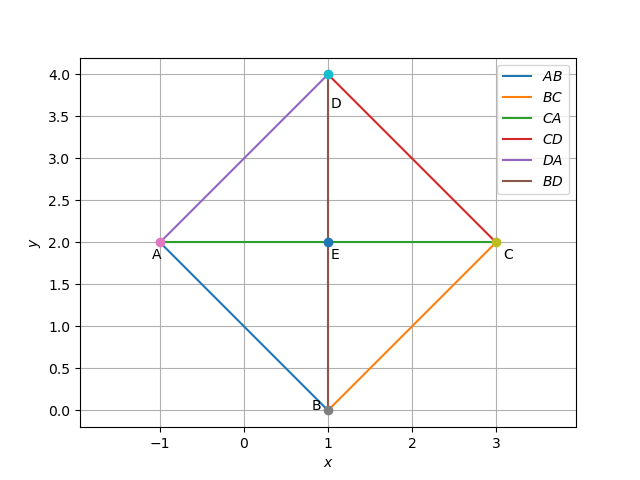
\includegraphics[width= \columnwidth]{solutions/1/4/quad.png}
\caption{Square ABCD}
\label{fig:2.2.7}
\end{figure}
See Fig. \ref{fig:2.2.7}.
The other two vertices can be obtained by using the following formula. 
\begin{align}
  \label{eq:square_points}
  \vec{B} = \frac{\norm{\vec{A}-\vec{C}}}{\sqrt{2}} \vec{P}\vec{e}_1+\vec{A}
  \\
  \vec{D} = \frac{\norm{\vec{A}-\vec{C}}}{\sqrt{2}} \vec{P}\vec{e}_2+\vec{A}
\end{align}
where 
\begin{align}
	\vec{P} = \myvec{\cos \brak{\theta-\frac{\pi}{4}} & \sin  \brak{\theta-\frac{\pi}{4}} \\ \sin \brak{\theta-\frac{\pi}{4}} & \cos \brak{\theta-\frac{\pi}{4}}}
\end{align}
and 



Let the given points be $\vec{A}, \vec{C}$.  The direction vector of the diagonal AC



\begin{enumerate}
\item From inspection we see that the opposite vertices forms a diagonal which is parallel to x-axis. Then the diagonal formed by other two vertices is parallel to y-axis(i.e. their x coordinates are equal). Let $\vec{A}= \myvec{-1\\2}$  and $\vec{C}=\myvec{3\\2}$. 

\item Diagonals bisect each other at 90\degree.
Let $\vec{B}$ and $\vec{D}$ be other two vertices. 
\item Using the property that diagonals bisect each other at 90\degree, we can obtain other vertices by rotating diagonal AC by 90\degree about $\vec{E}$ in clockwise or anticlockwise direction.

\item The rotation matrix for a rotation of angle 90\degree about origin in anticlockwise direction is given by
\begin{align}
\myvec{\cos90\degree&-\sin90\degree\\\sin90\degree&\cos90\degree}=\myvec{0&-1\\1&0}
\end{align}
The $\vec{E}$ is given by
\begin{align}
\vec{E}&= \frac{\vec{A}+\vec{C}}{2} \\
&= \myvec{1\\2}
\end{align}

\item To make the rotation we need to shift the $\vec{E}$ to origin. So the change in other vectors are
\begin{align}
\vec{A}-\vec{E}&=\myvec{-2\\0}\\
\vec{C}-\vec{E}&=\myvec{2\\0}
\end{align}

The required matrix now is $\myvec{-2&2\\0&0}$. Multiplying this with rotation matrix 
\begin{align}
&= \myvec{0&-1\\1&0}\myvec{-2&2\\0&0}\\
&=\myvec{0&0\\-2&2}
\end{align}
Now we obtained the coordinates as $\myvec{0\\-2}$ and $\myvec{0\\2}$.
To obtain the final coordinates we will add $\vec{E}$ to shift to the actual position.
\begin{align}
\vec{B}=\myvec{0\\-2}+\myvec{1\\2}\\
\vec{D}=\myvec{0\\2}+\myvec{1\\2}
\end{align}
Thus 
\begin{align}
\vec{B}&= \myvec{1\\0} \\
\vec{D}&= \myvec{1\\4}
\end{align} 
\item The python code for the figure can be downloaded from
\begin{lstlisting}
solutions/7/codes/quad/quad.py
\end{lstlisting}
\end{enumerate}  

%\input./solutions/point_vector/14/Latex/solution.tex}
\item Find a unit vector that makes an angle of $90\degree, 135\degree$ and $45\degree$ with the positive x, y and z axis respectively.
\solution 
%\input./solutions/point_vector/18/solution.tex}
\item If the lines
%
%
\begin{align}
\myvec{-3 & 1}\vec{x} &= 1
\\
\myvec{-1 & 2}\vec{x} &= 3
\end{align}
%
are equally inclined to the line
%
\begin{align}
\myvec{-m & 1}\vec{x} &= 4,
\end{align}
%
find the value of $m$.
%
\item In the following cases, determine whether the given planes are parallel or perpendicular, and in case they are neither, find the angles between them.
\begin{enumerate}
\item 
$
\myvec{7 & 5 & 6}\vec{x}=-30
$
 and 
$
\myvec{3 & -1 & -10}\vec{x}=-4
$
%
\item 
$
\myvec{2 & 1 & 3}\vec{x}=2
$
 and 
$
\myvec{1 & -2 & 5}\vec{x}=0
$
%
\item 
$
\myvec{2 & -2 & 4}\vec{x}=-5
$
 and 
$
\myvec{3 & -3 & 6}\vec{x}=1
$
\item 
$
\myvec{2 & -1 & 3}\vec{x}=1
$
 and 
$
\myvec{2 & -1 & 3}\vec{x}=-3
$
\item 
$
\myvec{4 & 8 & 1}\vec{x}=8
$
 and 
$
\myvec{0 & 1 & 1}\vec{x}=4
$
\end{enumerate}
\solution
\begin{enumerate}
    \item 
    %\input{solutions/su2021/2/43/b/main.tex}
    \item 
    %\input{solutions/su2021/2/43/c/ASSIGNMENT 5.tex}
    \item 
    %\input{solutions/su2021/2/43/d/main.tex}
    %
\end{enumerate}
\item Find the angle between the following pair of lines
\begin{enumerate}
\item 
\begin{align}
\frac{x-2}{2} = \frac{y-1}{5} &= \frac{z+3}{-3}, 
\\
\frac{x+2}{-1} = \frac{y-4}{8} &= \frac{z-5}{4} 
\end{align}
\item 
\begin{align}
\frac{x}{2} = \frac{y}{2} &= \frac{z}{1}, 
\\
\frac{x-5}{4} = \frac{y-2}{1} &= \frac{z-3}{8} 
\end{align}
\end{enumerate}
\solution
%\input{solutions/aug/2/34/88.tex}
\item A line makes angles $\alpha, \beta, \gamma, \delta$ with the diagonals of a cube, prove that \begin{align}
\cos^2\alpha + \cos^2\beta + \cos^2\gamma +\cos^2\delta = \frac{4}{3}.
\end{align}
\item Find the angle between the lines whose direction vectors are $\myvec{a& b &c}$ and $\myvec{b-c& c-a& a-b}$.
\item Find the angle between the vectors 
\begin{align}
\myvec{1\\-2\\3},
\myvec{3\\-2\\1}
\end{align}
\\
\solution 
%\input./solutions/point_vector/23/solution.tex}

\item Find the angle between the force $\vec{F} = \myvec{3\\4\\-5}$ and displacement $\vec{d} = \myvec{5\\4\\3}$.
%
\\
\solution 
%\input./solutions/point_vector/27/solution.tex}

\item Let $\norm{\vec{a}} = 3, \norm{\vec{b}}= 4, \norm{\vec{c}} = 5$ such that each vector is perpendicular to the other two.  Find $\norm{\vec{a}+\vec{b}+\vec{c}}$.
%
\\
\solution Given that 
%
\begin{align}
\label{eq:line_pair_orth}
 \vec{a}^T \vec{b} =  \vec{b}^T\vec{c}= \vec{c}^T\vec{a} = 0.
\end{align}
%
Then, 
%
\begin{multline}
\norm{\vec{a}+\vec{b}+\vec{c}}^2 = \norm{\vec{a}}^2+\norm{\vec{b}}^2+\norm{\vec{c}}^2
\\
+ \vec{a}^T \vec{b} +  \vec{b}^T\vec{c}+ \vec{c}^T\vec{a}.
\end{multline}
%
which reduces to 
%
\begin{align}
\norm{\vec{a}+\vec{b}+\vec{c}}^2 = \norm{\vec{a}}^2+\norm{\vec{b}}^2+\norm{\vec{c}}^2
\end{align}
%
using \eqref{eq:line_pair_orth}
%
\item Given 
\begin{align}
\label{eq:line_vec_sum_0}
 \vec{a}+\vec{b}+\vec{c} = \vec{0}, 
\end{align}
evaluate 
\begin{align}
 \vec{a}^T\vec{b}+\vec{b}^T\vec{c}+\vec{c}^T\vec{a},
\end{align}
given that $\norm{ \vec{a}}=3, \norm{ \vec{b}}= 4$ and $\norm{ \vec{c}} = 2 $.
%
\\
\solution Multiplying \eqref{eq:line_vec_sum_0} with $\vec{a}, \vec{b}, \vec{c}$,
\begin{align}
%\label{eq:line_vec_sum_0}
\norm{ \vec{a}}^2+\vec{a}^T\vec{b}+\vec{a}^T\vec{c} &= 0
\\
\vec{a}^T\vec{b}+\norm{ \vec{b}}^2+\vec{b}^T\vec{c} &= 0
\\
+\vec{c}^T\vec{a}+\vec{b}^T\vec{c}+\norm{ \vec{c}}^2 &= 0
\end{align}
%
Adding all the above equations and rearranging,
\begin{multline}
%\label{eq:line_vec_sum_0}
 \vec{a}^T\vec{b}+\vec{b}^T\vec{c}+\vec{c}^T\vec{a} = -\frac{\norm{ \vec{a}}^2+\norm{ \vec{b}}^2+\norm{ \vec{c}}^2}{2}
\end{multline}
\item Find the angle between the x-axis and the line joining the points \myvec{3\\–1} and \myvec{4\\–2}.
\solution
%\input./solutions/5/chapters/lines/docq9.tex}
\item Find the angle between the two planes
\label{prob:planes_angle}
\begin{align}
\myvec{2 & 1 & -2}\vec{x}&=5
\\
\myvec{3 &-6 & -2}\vec{x}&=7.
\end{align}
%
\solution The angle between two planes is the same as the angle between their normal vectors.  This can be obtained from \eqref{eq:line_scalar_prod}.

\item Find the angle between the two planes
\begin{align}
\myvec{2 & 2 & -2}\vec{x}&=5
\\
\myvec{3 &-6 & 2}\vec{x}&=7.
\end{align}
%
\solution See Problem \eqref{prob:planes_angle}.
%
\item Find the angle between the line 
%
\begin{align}
L: \quad \frac{x+1}{2} = \frac{y}{3} = \frac{z-3}{6} 
\end{align}
%
and
%
the plane 
\begin{align}
P: \quad \myvec{10 & 2 & -11}\vec{x}=3
\end{align}
%
\label{prob:plane_angle_line}
%
\solution The angle between the direction vector of $L$ and normal vector of $P$ is 
%
\begin{align}
\cos \theta &= \frac{\abs{\myvec{10 & 2 & -11}\myvec{2\\3\\6}}}{\sqrt{225}\times \sqrt{49}} = \frac{8}{21}
\end{align}
%
Thus, the desired angle is $90\degree -\theta$.
\item Find angles between the lines
\begin{align}
\myvec{\sqrt{3} & 1}\vec{x} &= 1
\\
\myvec{1 & \sqrt{3}}\vec{x} &= 1
\end{align}
\\
\solution
%\input{./solutions/line_plane/38/solution.tex}
\item Find the angle between the vectors 
$\vec{a}=\myvec{1\\1\\-1}$
  and 
$\vec{b}=\myvec{1\\-1\\1}$.
%
\\
\solution 
%\input{./solutions/line_exam/63/A1/latex/solution.tex}
%
\item Find the angle between the pair of lines given by 
\begin{align}
\vec{x} &= \myvec{3\\2\\-4} + \lambda_1\myvec{1 \\ 2 \\2}
\\
\vec{x} &= \myvec{5\\-2\\0} + \lambda_2\myvec{3 \\ 2 \\6}
\end{align}
%
\\
\solution 
%\input{./solutions/line_plane/64/Latex/solution.tex}
\item Find the angle between the pair of lines
\begin{align}
\frac{x+3}{3} = \frac{y-1}{5} &= \frac{z+3}{4}, 
\\
\frac{x+1}{1} = \frac{y-4}{1} &= \frac{z-5}{2} 
\end{align}
%
\\
\solution 
%\input{./solutions/line_exam/65/solution.tex}
%
\item Find the angle between two vectors $\vec{a}$ and $\vec{b}$ where 
%
\begin{align}
\norm{\vec{a}} = 1,
\norm{\vec{b}} = 2,
\vec{a}^T\vec{b} = 1.
\end{align}
%
\solution In Fig. \ref{fig:line_scalar_prod}, from the cosine formula, 
%
\begin{align}
\cos \theta &= \frac{\norm{\vec{A}-\vec{B}}^2+\norm{\vec{B}-\vec{C}}^2-\norm{\vec{A}-\vec{C}}^2}{2\norm{\vec{A}-\vec{B}}\norm{\vec{B}-\vec{C}}}
\end{align}
Letting $\vec{a} = \vec{A}-\vec{B}, \vec{b} = \vec{B}-\vec{C}$, 
\begin{align}
\cos \theta &= \frac{\norm{\vec{a}}^2+\norm{\vec{b}}^2-\norm{\vec{a}+\vec{b}}^2}{2\norm{\vec{a}}\norm{\vec{b}}}
\\
&= \frac{\norm{\vec{a}}^2+\norm{\vec{b}}^2-\sbrak{\norm{\vec{a}}^2+\norm{\vec{b}}^2-2\vec{a}^T\vec{b}}}{2\norm{\vec{a}}\norm{\vec{b}}}
\\
\implies \cos \theta &=\frac{\vec{a}^T\vec{b}}{\norm{\vec{a}}\norm{\vec{b}}}
\end{align}
%
Thus, the angle $\theta$ between two vectors is given by 
%
\begin{align}
\label{eq:line_scalar_prod}
\cos \theta &= \frac{\vec{a}^T\vec{b}}{\norm{\vec{a}}\norm{\vec{b}}}
\\
&=\frac{1}{2}
\\
\implies \theta &= 60\degree
\end{align}
%
%\begin{figure}[!ht]
%\includegraphics[width=\columnwidth]{./line/figs/line_scalar_prod.eps}
%\caption{}
%\label{fig:line_scalar_prod}
%\end{figure}
%


\item Find the angle between the lines 
%
\begin{align}
\myvec{1 & – \sqrt{3}}\vec{x}  = 5
\\
\myvec{\sqrt{3} & –1}\vec{x}  = -6
. 
\end{align}
%
\solution The angle between the lines can also be expressed in terms of the normal vectors as
%
\begin{align}
\cos \theta &= \frac{\vec{n}_1\vec{n}_2}{\norm{\vec{n}_1}\norm{\vec{n}_2}}
\\
&= \frac{\sqrt{3}}{2} \implies \theta = 30\degree
\end{align}
%
\item Find the angle between the planes whose equations are
$
\myvec{2 & 2 & -3}\vec{x}=5
$
 and 
$
\myvec{3 & -3 & 5}\vec{x}=3
$
\\
\solution
%\input{solutions/su2021/2/42/main.tex}
\item Find the angle between the following pair of lines:
\begin{align}
    L_1: \quad \vec{x} &= \myvec{3\\1\\-2} + \lambda_1\myvec{1 \\ -1 \\-2} \label{aug/22/eq:1} \\
    L_2: \quad \vec{x} &= \myvec{2\\-1\\-56} + \lambda_2\myvec{3 \\ -5 \\-4} \label{aug/22/eq:2}
    \end{align}
\solution
%\input{solutions/aug/22.tex}
\item Find the angle between the following pair of lines:
\begin{align}
L_1: \quad \vec{x} &= \myvec{2\\-5\\1} + \lambda_1\myvec{3 \\ 2 \\6}
\\
L_2: \quad \vec{x} &= \myvec{7\\-6\\0} + \lambda_2\myvec{1 \\ 2 \\2}
\end{align}
\\
\solution
%\input{./solutions/line_plane/73/solution.tex}
\item If the coordinates of the points $\bm{A}, \bm{B}, \bm{C}, \bm{D}$ be \myvec{1\\2\\3}, \myvec{4\\5\\7}, \myvec{-4\\3\\-6}, \myvec{2\\9\\2}, then find the angle between the lines $AB$ and $CD$.  
%
\\
\solution
%\input{solutions/aug/2/32/latex4.tex}
\end{enumerate}
\section{Orthogonality}
\renewcommand{\theequation}{\theenumi}
%\begin{enumerate}[label=\arabic*.,ref=\theenumi]
\begin{enumerate}[label=\thesection.\arabic*.,ref=\thesection.\theenumi]
\numberwithin{equation}{enumi}
\item Check whether 
\begin{align}
\myvec{5\\-2}, \myvec{6\\4}, \myvec{7\\-2}
\end{align}
are the vertices of an isosceles triangle.
%
\\
\solution
%\input{solutions/aug/2/5/EE3900 ASSIGNMENT-1.tex}
\item Show that each of the given three vectors is a unit vector
\begin{align}
 \frac{1}{7}\myvec{2\\3\\6}, \frac{1}{7}\myvec{3\\-6\\2}, \frac{1}{7}\myvec{6\\2\\-3}.
\end{align}
Also,  show that they are mutually perpendicular to each other.
\\
\solution 
%\input./solutions/point_vector/8/solution.tex}

\item For 
\begin{align}
\vec{a} = \myvec{2\\2\\3}, \vec{b} = \myvec{-1\\2\\1}, \vec{c} = \myvec{3\\1\\0},
\end{align}
$\brak{\vec{a}+k\vec{b}}\perp\vec{c}$.  Find $\lambda$.
\solution
%\input./solutions/point_vector/9/solution.tex}

\item Find ${\vec{a} \times \vec{b}}$ if 
\begin{align}
\vec{a}=\myvec{1\\-7\\7},
\vec{b}=\myvec{3\\-2\\2}.
\end{align}
\\
\solution 
%\input./solutions/point_vector/10/solution.tex}
\item The scalar product of \myvec{1\\1\\1} with a unit vector along the sum  of the vectors \myvec{2\\4\\-5} and \myvec{\lambda\\2\\3} is unity.  Find the value of $\lambda$.
\item The value of 
\begin{multline}
\myvec{1\\0\\0}^T\brak{\myvec{0\\1\\0}\times \myvec{0\\0\\1}}
+\myvec{0\\1\\0}^T\brak{\myvec{1\\0\\0}\times \myvec{0\\0\\1}}
\\
+\myvec{0\\0\\1}^T\brak{\myvec{1\\0\\0}\times \myvec{0\\1\\0}}
\end{multline}
%
is 
\begin{enumerate}[itemsep = 2pt]
\begin{multicols}{2}
\item 0
\item -1
\item 1
\item 3
\end{multicols}
\end{enumerate}
\solution 
%\input./solutions/point_vector/17/solution.tex}
\item Show that the lines with direction vectors \myvec{12\\-3\\-4}, \myvec{4\\12\\3} and \myvec{3\\-4\\12} are mutually perpendicular.
\item Show that the line through the points \myvec{1\\-1\\2}, \myvec{3\\4\\-2} is perpendicular to the line through the points   \myvec{0\\3\\2}, \myvec{3\\5\\6}.
\\
\solution 
%\input./solutions/point_vector/20/solution.tex}
\item If 
$\vec{a}=\myvec{5\\-1\\-3}$
  and 
$\vec{b}=\myvec{1\\3\\-5}$,
%
then show that the vectors $\vec{a}+\vec{b}$ and $\vec{a}-\vec{b}$ are perpendicular.
%
\\
\solution 
%\input./solutions/point_vector/66/latex/solution.tex}
\item Find the values of $p$ so that the lines 
\begin{align}
\frac{1-x}{3} = \frac{7y-14}{2p} &= \frac{z-3}{2}, 
\\
\frac{7-7x}{3p} = \frac{y-5}{1} &= \frac{6-z}{5} 
\end{align}
are at right angles.
\\
\solution
%\input{./solutions/line_plane/75/solution.tex}
\item Show that the lines 
\begin{align}
\frac{x-5}{7} = \frac{y+2}{-5} &= \frac{z}{1}, 
\\
\frac{x}{1} = \frac{y}{2} &= \frac{z}{3} 
\end{align}
%
are perpendicular to each other.
\\
\solution
%\input{./solutions/line_plane/76/solution.tex}
\item The line through the points \myvec{-2\\6} and \myvec{4\\8} is perpendicular to the line through the points \myvec{8\\12} and $\myvec{x\\24}$.  Find the value of $x$.
\\
\solution
%\input{solutions/su2021/2/36/main.tex}
\item Show that the line joining the origin to the point \myvec{2\\1\\1} is perpendicular to the line determined by the points \myvec{3\\5\\-1}, \myvec{4\\3\\-1}.
\\
\solution
%\input{solutions/su2021/2/37.tex}
\item Are the points 
\begin{align}
\vec{A} = \myvec{3\\6 \\9},
\vec{B} = \myvec{10\\20 \\30},
\vec{C} = \myvec{25\\ -41\\5},
\end{align}
%
the vertices of a right angled triangle?
\\
\solution
%\input{solutions/july/2/6/Assignment4.tex}
\item Show that the vectors 
$
\myvec{2\\-1 \\1},
\myvec{1\\-3 \\-5},
\myvec{3\\ -4\\-4}
$
form the vertices of a right angled triangle.
\\
\solution
%\input{solutions/aug/2/3/Assignment-1.tex}
\item Show that the points 
\begin{align}
\vec{A} = \myvec{2\\-1 \\1},
\vec{B} = \myvec{1\\-3 \\-5},
\vec{C} = \myvec{3\\ -4\\-4}
\end{align}
%
are the vertices of a right angled triangle.
\\
\solution
%\input{solutions/su2021/2/4/Assignment 8 (3).tex}


\item In $\triangle ABC$, 
$
\vec{A} = \myvec{1\\2 \\3},
\vec{B} = \myvec{-1\\0 \\0},
\vec{C} = \myvec{0\\ 1\\2}.
$
Find $\angle B$.
\\
\solution
%\input{solutions/su2021/2/5/main.tex}
\item Without using the Pythagoras theorem, show that the points \myvec{4\\ 4}, \myvec{3\\ 5} and \myvec{–1\\ –1} are the vertices of a right angled triangle.
\\
\solution
%\input{./solutions/triangle/18/solution.tex}
\item Show that the points 
\begin{align}
\vec{A} = \myvec{2\\-1 \\1},
\vec{B} = \myvec{1\\-3 \\-5},
\vec{C} = \myvec{3\\ -4\\-4}
\end{align}
%
are the vertices of a right angled triangle.
\\
\solution 
The following code plots Fig. \ref{fig:triangle_3d}
%
\begin{lstlisting}
codes/triangle/triangle_3d.py
\end{lstlisting}
%
%\begin{figure}[!ht]
%\includegraphics[width=\columnwidth]{./triangle/figs/triangle_3d.eps}
%\caption{}
%\label{fig:triangle_3d}
%\end{figure}
%
From the figure, it appears that $\triangle ABC$ is right angled at $\vec{C}$.  Since 
\begin{align}
\brak{\vec{A}-\vec{C}}^T\brak{\vec{B}-\vec{C}}&=0
\end{align}
%
it is proved that the triangle is indeed right angled.
\item Show that the points $\vec{A} = \myvec{1\\7}, \vec{B} = \myvec{4\\2}, \vec{C}=\myvec{-1\\-1},\vec{D}= \myvec{-4\\4} $  are the vertices of a square.
\\
\solution By inspection, 
%
\begin{align}
\frac{\vec{A}+\vec{C}}{2}=\frac{\vec{B}+\vec{D}}{2} = \myvec{0\\3}
\end{align}
%
Hence, the diagonals $AC$ and $BD$ bisect each other.
%
Also, 
\begin{align}
\brak{\vec{A}-\vec{C}}^T
\brak{\vec{B}-\vec{D}} = 0
\end{align}
%
$\implies AC \perp BD $.  Hence $ABCD$ is a square.
\item Show that the points 
$\vec{A} = \myvec{1\\2\\3},
 \vec{B} = \myvec{-1\\-2\\-1},
\vec{C} = \myvec{2\\3\\2},
\vec{D} = \myvec{4\\7\\6}.
$
are the vertices of a parallelogram $ABCD$ but it is not a rectangle.
%
\\
\solution Since the direction vectors
%
\begin{align}
\vec{A}-\vec{B}&= \vec{D}-\vec{C}
\\
\vec{A}-\vec{D}&= \vec{B}-\vec{C}
\end{align}
%
$AB \parallel CD$ and $AD \parallel BC$.  Hence $ABCD$ is a parallelogram.  However, 
%
\begin{align}
\brak{\vec{A}-\vec{B}}^T\brak{ \vec{A}-\vec{D}}\ne 0
\end{align}
%
Hence, it is not a rectangle.
The following code plots Fig. \ref{fig:quad_3d}
%
\begin{lstlisting}
codes/triangle/quad_3d.py
\end{lstlisting}
%
%\begin{figure}[!ht]
%\includegraphics[width=\columnwidth]{./triangle/figs/quad_3d.eps}
%\caption{}
%\label{fig:quad_3d}
%\end{figure}
%

\item $ABCD$ is a rectangle formed by the points $\vec{A} = \myvec{-1\\-1}, \vec{B} = \myvec{-1\\4}, \vec{C} = \myvec{5\\4}, \vec{D} = \myvec{5\\-1}$. $ \vec{P}, \vec{Q}, \vec{R}, \vec{S}$ are the mid points of $AB, BC, CD, DA$ respectively.  Is the quadrilateral $PQRS$ a 
\begin{enumerate}
\item square?
\item rectangle?
\item rhombus?
\end{enumerate}
\solution
%\input{./solutions/quad/1/solution}
\end{enumerate}

\section{Projection}
\renewcommand{\theequation}{\theenumi}
%\begin{enumerate}[label=\arabic*.,ref=\theenumi]
\begin{enumerate}[label=\thesection.\arabic*.,ref=\thesection.\theenumi]
\numberwithin{equation}{enumi}
\item Find the projection of the vector 
\begin{align}
\myvec{1\\3\\7}
\end{align}
on the vector
\begin{align}
\myvec{7\\-1\\8}
\end{align}
\\
\solution 
%\input./solutions/point_vector/24/solution.tex}
\item Find the projection of the vector 
\begin{align}
\vec{a} = \myvec{2\\3\\2}
\end{align}
on the vector
\begin{align}
\vec{b}=\myvec{1\\2\\1}.
\end{align}
%
\solution The projection of $\vec{a}$ on $\vec{b}$ is shown in Fig. \ref{fig:line_proj}. It has magnitude $\norm{\vec{a}}\cos \theta$ and is in the direction of $\vec{b}$.
%
%
%\begin{figure}
%\centering
%\includegraphics[width=\columnwidth]{./line/figs/line_proj.eps}
%\caption{}
%\label{fig:line_proj}
%\end{figure}
%
Thus, the projection is defined as 
\begin{align}
\brak{\norm{\vec{a}}\cos\theta} \frac{\vec{b}}{\norm{\vec{b}}}
=  \frac{\brak{\vec{a}^T\vec{b}}\norm{\vec{a}}}{\norm{\vec{b}}}\vec{b}
\end{align}
\end{enumerate}
\section{Affine Transformation}
\renewcommand{\theequation}{\theenumi}
%\begin{enumerate}[label=\arabic*.,ref=\theenumi]
\begin{enumerate}[label=\thesection.\arabic*.,ref=\thesection.\theenumi]
\numberwithin{equation}{enumi}
\item The two opposite vertices of a square are \myvec{-1\\2},  \myvec{3\\2}. Find the coordinates of the other two vertices.
\\
\solution
\begin{figure}[!ht]
\centering
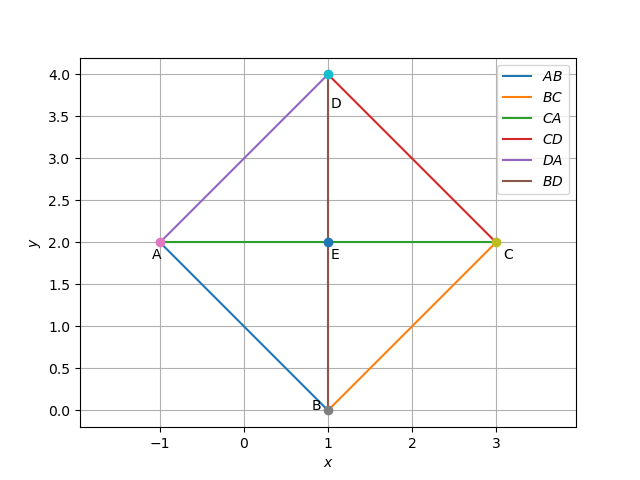
\includegraphics[width= \columnwidth]{solutions/1/4/quad.png}
\caption{Square ABCD}
\label{fig:2.2.7}
\end{figure}
See Fig. \ref{fig:2.2.7}.
The other two vertices can be obtained by using the following formula. 
\begin{align}
  \label{eq:square_points}
  \vec{B} = \frac{\norm{\vec{A}-\vec{C}}}{\sqrt{2}} \vec{P}\vec{e}_1+\vec{A}
  \\
  \vec{D} = \frac{\norm{\vec{A}-\vec{C}}}{\sqrt{2}} \vec{P}\vec{e}_2+\vec{A}
\end{align}
where 
\begin{align}
	\vec{P} = \myvec{\cos \brak{\theta-\frac{\pi}{4}} & \sin  \brak{\theta-\frac{\pi}{4}} \\ \sin \brak{\theta-\frac{\pi}{4}} & \cos \brak{\theta-\frac{\pi}{4}}}
\end{align}
and 



Let the given points be $\vec{A}, \vec{C}$.  The direction vector of the diagonal AC



\begin{enumerate}
\item From inspection we see that the opposite vertices forms a diagonal which is parallel to x-axis. Then the diagonal formed by other two vertices is parallel to y-axis(i.e. their x coordinates are equal). Let $\vec{A}= \myvec{-1\\2}$  and $\vec{C}=\myvec{3\\2}$. 

\item Diagonals bisect each other at 90\degree.
Let $\vec{B}$ and $\vec{D}$ be other two vertices. 
\item Using the property that diagonals bisect each other at 90\degree, we can obtain other vertices by rotating diagonal AC by 90\degree about $\vec{E}$ in clockwise or anticlockwise direction.

\item The rotation matrix for a rotation of angle 90\degree about origin in anticlockwise direction is given by
\begin{align}
\myvec{\cos90\degree&-\sin90\degree\\\sin90\degree&\cos90\degree}=\myvec{0&-1\\1&0}
\end{align}
The $\vec{E}$ is given by
\begin{align}
\vec{E}&= \frac{\vec{A}+\vec{C}}{2} \\
&= \myvec{1\\2}
\end{align}

\item To make the rotation we need to shift the $\vec{E}$ to origin. So the change in other vectors are
\begin{align}
\vec{A}-\vec{E}&=\myvec{-2\\0}\\
\vec{C}-\vec{E}&=\myvec{2\\0}
\end{align}

The required matrix now is $\myvec{-2&2\\0&0}$. Multiplying this with rotation matrix 
\begin{align}
&= \myvec{0&-1\\1&0}\myvec{-2&2\\0&0}\\
&=\myvec{0&0\\-2&2}
\end{align}
Now we obtained the coordinates as $\myvec{0\\-2}$ and $\myvec{0\\2}$.
To obtain the final coordinates we will add $\vec{E}$ to shift to the actual position.
\begin{align}
\vec{B}=\myvec{0\\-2}+\myvec{1\\2}\\
\vec{D}=\myvec{0\\2}+\myvec{1\\2}
\end{align}
Thus 
\begin{align}
\vec{B}&= \myvec{1\\0} \\
\vec{D}&= \myvec{1\\4}
\end{align} 
\item The python code for the figure can be downloaded from
\begin{lstlisting}
solutions/7/codes/quad/quad.py
\end{lstlisting}
\end{enumerate}  

\end{enumerate}
\section{Application}
\renewcommand{\theequation}{\theenumi}
%\begin{enumerate}[label=\arabic*.,ref=\theenumi]
\begin{enumerate}[label=\thesection.\arabic*.,ref=\thesection.\theenumi]
\numberwithin{equation}{enumi}
\item If $\theta$ is the angle between two vectors $\vec{a}$ and $\vec{b}$, then $\vec{a}^T\vec{b} \ge $ only when 
\begin{enumerate}[itemsep = 2pt]
\begin{multicols}{2}
\item $0 < \theta < \frac{\pi}{2}$
\item $0 \le \theta \le \frac{\pi}{2}$
\item $0 < \theta < {\pi}$
\item $0 \le \theta \le {\pi}$
\end{multicols}
\end{enumerate}
\item Let $\vec{a}$ and $\vec{b}$ be two unit vectors and $\theta$ be the angle between them.  Then $\vec{a}+\vec{b}$ is a unit vector if 
\begin{enumerate}[itemsep = 2pt]
\begin{multicols}{2}
\item $\theta = \frac{\pi}{4}$
\item $\theta = \frac{\pi}{3}$
\item $\theta = \frac{\pi}{2}$
\item $\theta = \frac{2\pi}{3}$
\end{multicols}
\end{enumerate}
\item If $\theta$ is the angle between any two vectors $\vec{a}$ and $\vec{b}$, then 
$\norm{\vec{a}^T\vec{b}} = \norm{\vec{a} \times \vec{b}}$ when $\theta$ is equal to 
\begin{enumerate}[itemsep = 2pt]
\begin{multicols}{2}
\item 0
\item $\frac{\pi}{4}$
\item $\frac{\pi}{2}$
\item $\pi$.
\end{multicols}
\end{enumerate}
\item Show that 
\begin{align}
\brak{\norm{\vec{a}}\vec{b}+\norm{\vec{b}}\vec{a}}\perp \brak{\norm{\vec{a}}\vec{b}-\norm{\vec{b}}\vec{a}}\\
\end{align}
\item Find $\norm{\vec{a}}$ and $\norm{\vec{b}}$, if
\begin{align}
\norm{\vec{a}} &= \norm{\vec{b}},
\\
\vec{a}^T\vec{b} = \frac{1}{2} 
\end{align}
and the angle between $\vec{a}$ and $\vec{b}$ is $60\degree$.
\item Let $\bm{\alpha} = \myvec{3\\-1\\0}, \bm{\beta} = \myvec{2\\1\\-3}$.  Find $\bm{\beta}_1, \bm{\beta}_2 $ such that $\bm{\beta}=\bm{\beta}_1+\bm{\beta}_2, \bm{\beta}_1 \parallel  \bm{\alpha} $ and $\bm{\beta}_2 \perp \bm{\alpha} $.
%
\label{prob:line_gram_schmidt}
\\
\solution Let $\beta_1 = k\alpha$.  Then, 
%
\begin{align}
\bm{\beta} &= k\bm{\alpha}+\bm{\beta}_2
\\
\implies k &= \frac{\bm{\alpha}^T\bm{\beta}}{\norm{\bm{\alpha}}^2}
\end{align}
%
and 
%
\begin{align}
\bm{\beta}_2 &= \bm{\beta}-k\bm{\alpha}
\end{align}
%
This process is known as {\em Gram-Schmidth orthogonalization}.

\item A body constrained to move along the z-axis of a coordinate system is subject to a constant force
\begin{align}
\vec{F} = \myvec{-1\\2\\3}
\end{align}
%
What is the work done by this force in moving the body a distance of 4 m along the z-axis ?
\\
\solution 
%\input./solutions/point_vector/28/solution.tex}
\end{enumerate}
\end{document}


